% Graphic: Brute force binary combinations
\begin{figure}[H]
    \centering
    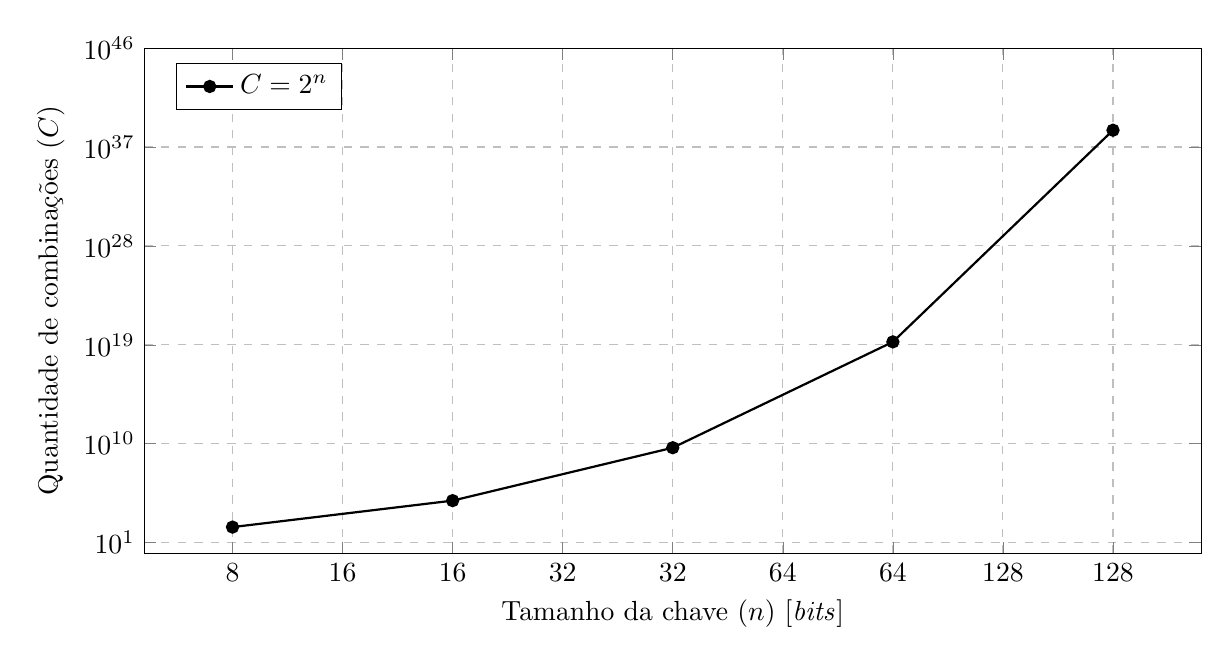
\begin{tikzpicture}
        \begin{semilogyaxis}[
            % title={Combinações possíveis para chaves binárias},
            xlabel={Tamanho da chave ($n$) [\textit{bits}]}, %aqui, por algum motivo, a constante \bits ficou com espaco extra no final
            ylabel={Quantidade de combinações ($C$)},
            ymin=1, ymax=10^46,
            symbolic x coords={8,16,32,64,128},
            legend pos=north west,
            ymajorgrids=true,
            xmajorgrids=true,
            grid style=dashed,
            height=8cm,
            width=15cm
        ]
     
        \addplot[color=black, solid, thick, mark=*]
            coordinates {
                (8,   256)                                     %   8 bits
                (16,  65536)                                   %  16 bits
                (32,  4294967296)                              %  32 bits
                (64,  18446744070000000000)                    %  64 bits
                (128, 340282366900000000000000000000000000000) % 128 bits
            };
            \legend{$C = 2^n$}
     
        \end{semilogyaxis}
    \end{tikzpicture}
    \caption{Quantidade de combinações possíveis para chaves binárias.}
    \label{graph:combinations}
\end{figure}